%!TEX TS-program = xelatex

% Шаблон документа LaTeX создан в 2018 году
% Алексеем Подчезерцевым
% В качестве исходных использованы шаблоны
% 	Данилом Фёдоровых (danil@fedorovykh.ru) 
%		https://www.writelatex.com/coursera/latex/5.2.2
%	LaTeX-шаблон для русской кандидатской диссертации и её автореферата.
%		https://github.com/AndreyAkinshin/Russian-Phd-LaTeX-Dissertation-Template

\documentclass[a4paper,14pt]{article}


%%% Работа с русским языком
\usepackage[english,russian]{babel}   %% загружает пакет многоязыковой вёрстки
\usepackage{fontspec}      %% подготавливает загрузку шрифтов Open Type, True Type и др.
\defaultfontfeatures{Ligatures={TeX},Renderer=Basic}  %% свойства шрифтов по умолчанию
\setmainfont[Ligatures={TeX,Historic}]{Times New Roman} %% задаёт основной шрифт документа
\setsansfont{Comic Sans MS}                    %% задаёт шрифт без засечек
\setmonofont{Courier New}
\usepackage{indentfirst}
\frenchspacing

\renewcommand{\epsilon}{\ensuremath{\varepsilon}}
\renewcommand{\phi}{\ensuremath{\varphi}}
\renewcommand{\kappa}{\ensuremath{\varkappa}}
\renewcommand{\le}{\ensuremath{\leqslant}}
\renewcommand{\leq}{\ensuremath{\leqslant}}
\renewcommand{\ge}{\ensuremath{\geqslant}}
\renewcommand{\geq}{\ensuremath{\geqslant}}
\renewcommand{\emptyset}{\varnothing}

%%% Дополнительная работа с математикой
\usepackage{amsmath,amsfonts,amssymb,amsthm,mathtools} % AMS
\usepackage{icomma} % "Умная" запятая: $0,2$ --- число, $0, 2$ --- перечисление

%% Номера формул
%\mathtoolsset{showonlyrefs=true} % Показывать номера только у тех формул, на которые есть \eqref{} в тексте.
%\usepackage{leqno} % Нумерация формул слева	

%% Перенос знаков в формулах (по Львовскому)
\newcommand*{\hm}[1]{#1\nobreak\discretionary{}
	{\hbox{$\mathsurround=0pt #1$}}{}}

%%% Работа с картинками
\usepackage{graphicx}  % Для вставки рисунков
\graphicspath{{images/}}  % папки с картинками
\setlength\fboxsep{3pt} % Отступ рамки \fbox{} от рисунка
\setlength\fboxrule{1pt} % Толщина линий рамки \fbox{}
\usepackage{wrapfig} % Обтекание рисунков текстом

%%% Работа с таблицами
\usepackage{array,tabularx,tabulary,booktabs} % Дополнительная работа с таблицами
\usepackage{longtable}  % Длинные таблицы
\usepackage{multirow} % Слияние строк в таблице
\usepackage{float}% http://ctan.org/pkg/float

%%% Программирование
\usepackage{etoolbox} % логические операторы


%%% Страница
\usepackage{extsizes} % Возможность сделать 14-й шрифт
\usepackage{geometry} % Простой способ задавать поля
\geometry{top=20mm}
\geometry{bottom=20mm}
\geometry{left=20mm}
\geometry{right=10mm}
%
%\usepackage{fancyhdr} % Колонтитулы
% 	\pagestyle{fancy}
%\renewcommand{\headrulewidth}{0pt}  % Толщина линейки, отчеркивающей верхний колонтитул
% 	\lfoot{Нижний левый}
% 	\rfoot{Нижний правый}
% 	\rhead{Верхний правый}
% 	\chead{Верхний в центре}
% 	\lhead{Верхний левый}
%	\cfoot{Нижний в центре} % По умолчанию здесь номер страницы

\usepackage{setspace} % Интерлиньяж
\onehalfspacing % Интерлиньяж 1.5
%\doublespacing % Интерлиньяж 2
%\singlespacing % Интерлиньяж 1

\usepackage{lastpage} % Узнать, сколько всего страниц в документе.

\usepackage{soul} % Модификаторы начертания

\usepackage{hyperref}
\usepackage[usenames,dvipsnames,svgnames,table,rgb]{xcolor}
\hypersetup{				% Гиперссылки
	unicode=true,           % русские буквы в раздела PDF
	pdftitle={Практическая по БД},   % Заголовок
	pdfauthor={Подчезерцев Алексей},      % Автор
	pdfsubject={Создание и заполнение отношений БД фитнес-клуба},      % Тема
	pdfcreator={Подчезерцев Алексей}, % Создатель
	pdfproducer={Подчезерцев Алексей}, % Производитель
	pdfkeywords={БД} {SQL} {MySQL}, % Ключевые слова
	colorlinks=true,       	% false: ссылки в рамках; true: цветные ссылки
	linkcolor=black,          % внутренние ссылки
	citecolor=black,        % на библиографию
	filecolor=magenta,      % на файлы
	urlcolor=black           % на URL
}
\makeatletter 
\def\@biblabel#1{#1. } 
\makeatother
\usepackage{cite} % Работа с библиографией
%\usepackage[superscript]{cite} % Ссылки в верхних индексах
%\usepackage[nocompress]{cite} % 
\usepackage{csquotes} % Еще инструменты для ссылок

\usepackage{multicol} % Несколько колонок

\usepackage{tikz} % Работа с графикой
\usepackage{pgfplots}
\usepackage{pgfplotstable}

% ГОСТ заголовки
\usepackage[font=small]{caption}
%\captionsetup[table]{justification=centering, labelsep = newline} % Таблицы по правобу краю
%\captionsetup[figure]{justification=centering} % Картинки по центру


\newcommand{\tablecaption}[1]{\addtocounter{table}{1}\small \begin{flushright}\tablename \ \thetable\end{flushright}%	
\begin{center}#1\end{center}}

\newcommand{\imref}[1]{Рис.~\ref{#1}}

\usepackage{multirow}
\usepackage{spreadtab}
\newcolumntype{K}[1]{@{}>{\centering\arraybackslash}p{#1cm}@{}}


\usepackage{xparse}
\ExplSyntaxOn
\DeclareExpandableDocumentCommand{\juliandate}{ m m m }
{
	\juliandate_calc:nnnn { #1 } { #2 } { #3 } { \use:n }
}
\NewDocumentCommand{\storejuliandate}{ s m m m m }
{
	\IfBooleanTF{#1}
	{
		\juliandate_calc:nnnn { #3 } { #4 } { #5 } { \cs_set:Npx #2 }
	}
	{
		\juliandate_calc:nnnn { #3 } { #4 } { #5 } { \cs_new:Npx #2 }
	}
}
\cs_new:Npn \juliandate_calc:nnnn #1 #2 #3 #4 % #1 = day, #2 = month, #3 = year, #4 = what to do
{
	#4 
	{
		\int_eval:n
		{
			#1 +
			\int_div_truncate:nn { 153 * (#2 + 12 * \int_div_truncate:nn { 14 - #2 } { 12 } - 3) + 2 } { 5 } +
			365 * (#3 + 4800 - \int_div_truncate:nn { 14 - #2 } { 12 } ) +
			\int_div_truncate:nn { #3 + 4800 - \int_div_truncate:nn { 14 - #2 } { 12 } } { 4 } -
			\int_div_truncate:nn { #3 + 4800 - \int_div_truncate:nn { 14 - #2 } { 12 } } { 100 } + 
			\int_div_truncate:nn { #3 + 4800 - \int_div_truncate:nn { 14 - #2 } { 12 } } { 400 } -
			32045
		}
	}
}

\tl_new:N \l__juliandate_g_tl
\tl_new:N \l__juliandate_dg_tl
\tl_new:N \l__juliandate_c_tl
\tl_new:N \l__juliandate_dc_tl
\tl_new:N \l__juliandate_b_tl
\tl_new:N \l__juliandate_db_tl
\tl_new:N \l__juliandate_a_tl
\tl_new:N \l__juliandate_da_tl
\tl_new:N \l__juliandate_y_tl
\tl_new:N \l__juliandate_m_tl
\tl_new:N \l__juliandate_d_tl
\int_new:N \l_juliandate_day_int
\int_new:N \l_juliandate_month_int
\int_new:N \l_juliandate_year_int

\cs_new:Npn \__juliandate_set:nn #1 #2
{
	\tl_set:cx { l__juliandate_#1_tl } { \int_eval:n { #2 } }
}
\cs_new:Npn \__juliandate_use:n #1
{
	\tl_use:c { l__juliandate_#1_tl }
}
\cs_new_protected:Npn \juliandate_reverse:n #1
{
	\__juliandate_set:nn { g }
	{ \int_div_truncate:nn { #1 + 32044 } { 146097 } }
	\__juliandate_set:nn { dg }
	{ \int_mod:nn { #1 + 32044 } { 146097 } }
	\__juliandate_set:nn { c }
	{ \int_div_truncate:nn { ( \int_div_truncate:nn { \__juliandate_use:n { dg } } { 36524 } + 1) * 3 } { 4 } }
	\__juliandate_set:nn { dc }
	{ \__juliandate_use:n { dg } - \__juliandate_use:n { c } * 36524 }
	\__juliandate_set:nn { b }
	{ \int_div_truncate:nn { \__juliandate_use:n { dc } } { 1461 } }
	\__juliandate_set:nn { db }
	{ \int_mod:nn { \__juliandate_use:n { dc } } { 1461 } }
	\__juliandate_set:nn { a }
	{ \int_div_truncate:nn { ( \int_div_truncate:nn { \__juliandate_use:n { db } } { 365 } + 1) * 3 } { 4 } }
	\__juliandate_set:nn { da }
	{ \__juliandate_use:n { db } - \__juliandate_use:n { a } * 365 }
	\__juliandate_set:nn { y }
	{
		\__juliandate_use:n { g } * 400 + 
		\__juliandate_use:n { c } * 100 + 
		\__juliandate_use:n { b } * 4 + 
		\__juliandate_use:n { a }
	}
	\__juliandate_set:nn { m }
	{ \int_div_truncate:nn { \__juliandate_use:n { da } * 5 + 308 } { 153 } - 2 }
	\__juliandate_set:nn { d }
	{ \__juliandate_use:n { da } - \int_div_truncate:nn { (\__juliandate_use:n { m } + 4) * 153 } { 5 } + 122 }
	\int_set:Nn \l_juliandate_year_int
	{ \__juliandate_use:n { y } - 4800 + \int_div_truncate:nn { \__juliandate_use:n { m } + 2 } { 12 } }
	\int_set:Nn \l_juliandate_month_int
	{ \int_mod:nn { \__juliandate_use:n { m } + 2 } { 12 } + 1 }
	\int_set:Nn \l_juliandate_day_int
	{ \__juliandate_use:n { d } + 1 }
}
\cs_generate_variant:Nn \juliandate_reverse:n { x }

\NewDocumentCommand{\showday}{ m }
{
	\juliandate_reverse:n { #1 }
	\int_to_arabic:n { \l_juliandate_day_int }-
	\int_to_arabic:n { \l_juliandate_month_int }-
	\int_to_arabic:n { \l_juliandate_year_int }
}

\NewDocumentCommand{\tomorrow}{ }
{
	\group_begin:
	\juliandate_reverse:x { \juliandate_calc:nnnn { \day + 1 } { \month } { \year } { \use:n } }
	\day = \l_juliandate_day_int
	\month = \l_juliandate_month_int
	\year = \l_juliandate_year_int
	\today
	\group_end:
}
\NewDocumentCommand{\tomorrowof}{ m m m }
{
	\group_begin:
	\juliandate_reverse:x { \juliandate_calc:nnnn { #1 + 1 } { #2 } { #3 } { \use:n } }
	\day = \l_juliandate_day_int
	\month = \l_juliandate_month_int
	\year = \l_juliandate_year_int
	\today
	\group_end:
}
\ExplSyntaxOff


\usepackage{xcolor,listings}
\usepackage{textcomp}
\begin{document} % конец преамбулы, начало документа
\begin{titlepage}
	\begin{center}
		ФЕДЕРАЛЬНОЕ  ГОСУДАРСТВЕННОЕ АВТОНОМНОЕ \\
		ОБРАЗОВАТЕЛЬНОЕ УЧРЕЖДЕНИЕ ВЫСШЕГО ОБРАЗОВАНИЯ\\
		«НАЦИОНАЛЬНЫЙ ИССЛЕДОВАТЕЛЬСКИЙ УНИВЕРСИТЕТ\\
		«ВЫСШАЯ ШКОЛА ЭКОНОМИКИ»
	\end{center}
	
	\begin{center}
		\textbf{Московский институт электроники и математики}
		
		\textbf{Им. А.Н.Тихонова НИУ ВШЭ}
		
		\textbf{Департамент электронной инженерии}
	\end{center}	
	\vspace{5ex}
	\begin{center}
\textbf{<<ПОЛУЧЕНИЕ, ОБРАБОТКА И ПРЕДСТАВЛЕНИЕ РЕЗУЛЬТАТОВ МНОГОКРАТНЫХ ИЗМЕРЕНИЙ>>}
	\end{center}	
	\vspace{1ex}
	\begin{center}
\textbf{Отчёт по части 2 лабораторного практикума по дисциплине \\
	<<Электротехника, электроника и метрология>>, раздел <<Метрология>>(ЛР 5-7)}
	\end{center}	
	\vspace{5ex}
	
	\begin{multicols}{2}
	\vfill\null
	\columnbreak
	ВЫПОЛНИЛИ:
	
	Подчезерцев Алексей Евгеньевич
	
	Солодянкин Андрей Александрович
	
	группа БИВ172
	\end{multicols}

	\vfill
	\begin{center}
		Москва \the\year
	\end{center}
\end{titlepage}
\tableofcontents
\pagebreak
\section{Цели работы}
\begin{itemize}
	\item Экспериментальное Исследование входных и выходных вольт-амперных характеристик (ВАХ) биполярного транзистора.
	
	\item Приобретение навыков измерения характеристик биполярных транзисторов и  определения основных параметров схемотехнической модели Гуммеля-Пуна транзистора по резкльтатам измерения его ВАХ.
	
	\item Приобретение навыков расчета схем и моднлирование характеристик транзисторов с помощью программы схемотехнического моделированря SPICE.
\end{itemize}

\section{Теоретическое введение}

\begin{figure}[H]
	\centering
	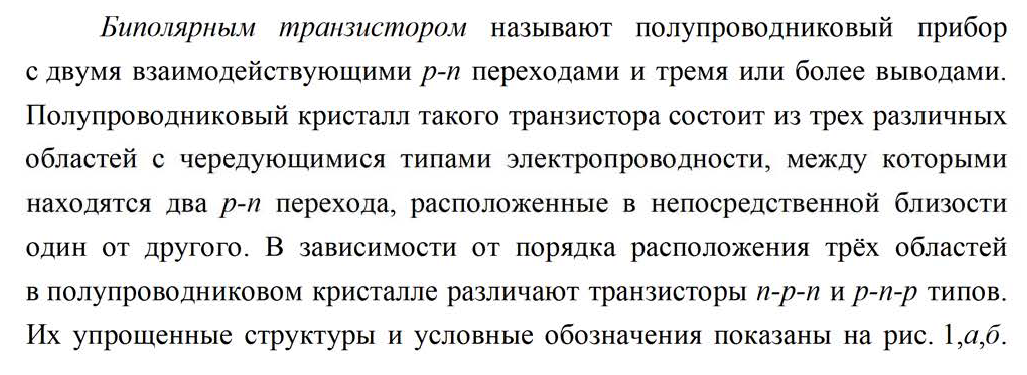
\includegraphics[width=\linewidth]{images/theory_1}
	\caption*{}
	\label{fig:theory1}
\end{figure}

\begin{figure}[H]
	\centering
	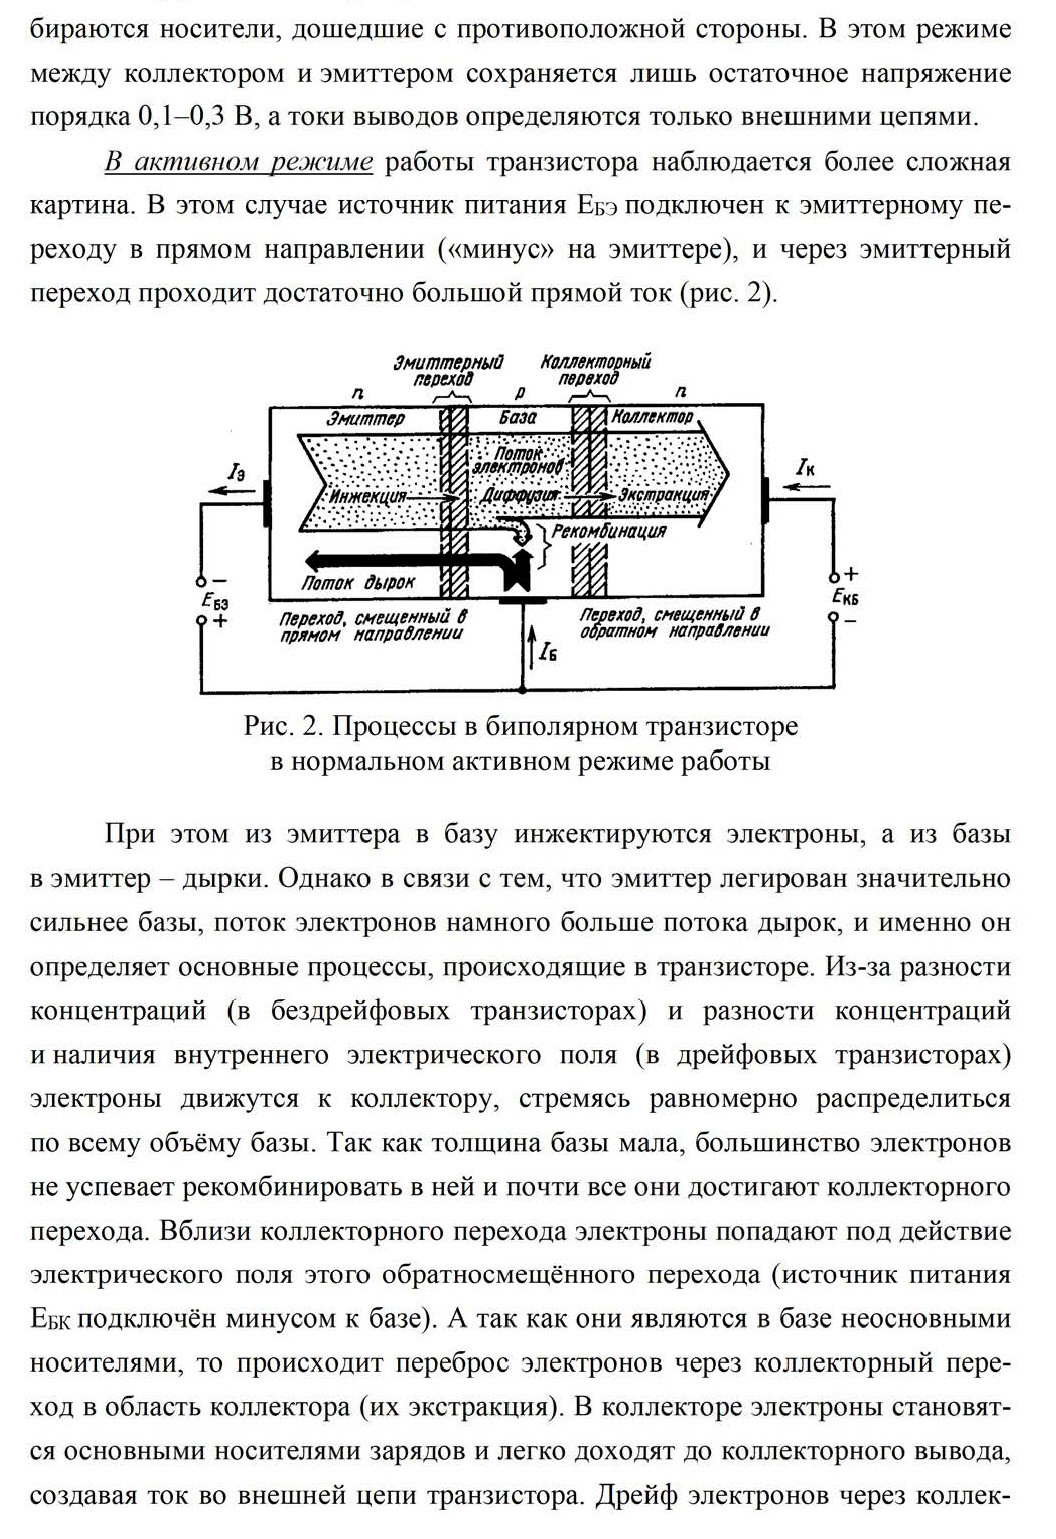
\includegraphics[width=\linewidth]{images/theory_2}
	\caption*{}
	\label{fig:theory2}
\end{figure}

\begin{figure}[H]
	\centering
	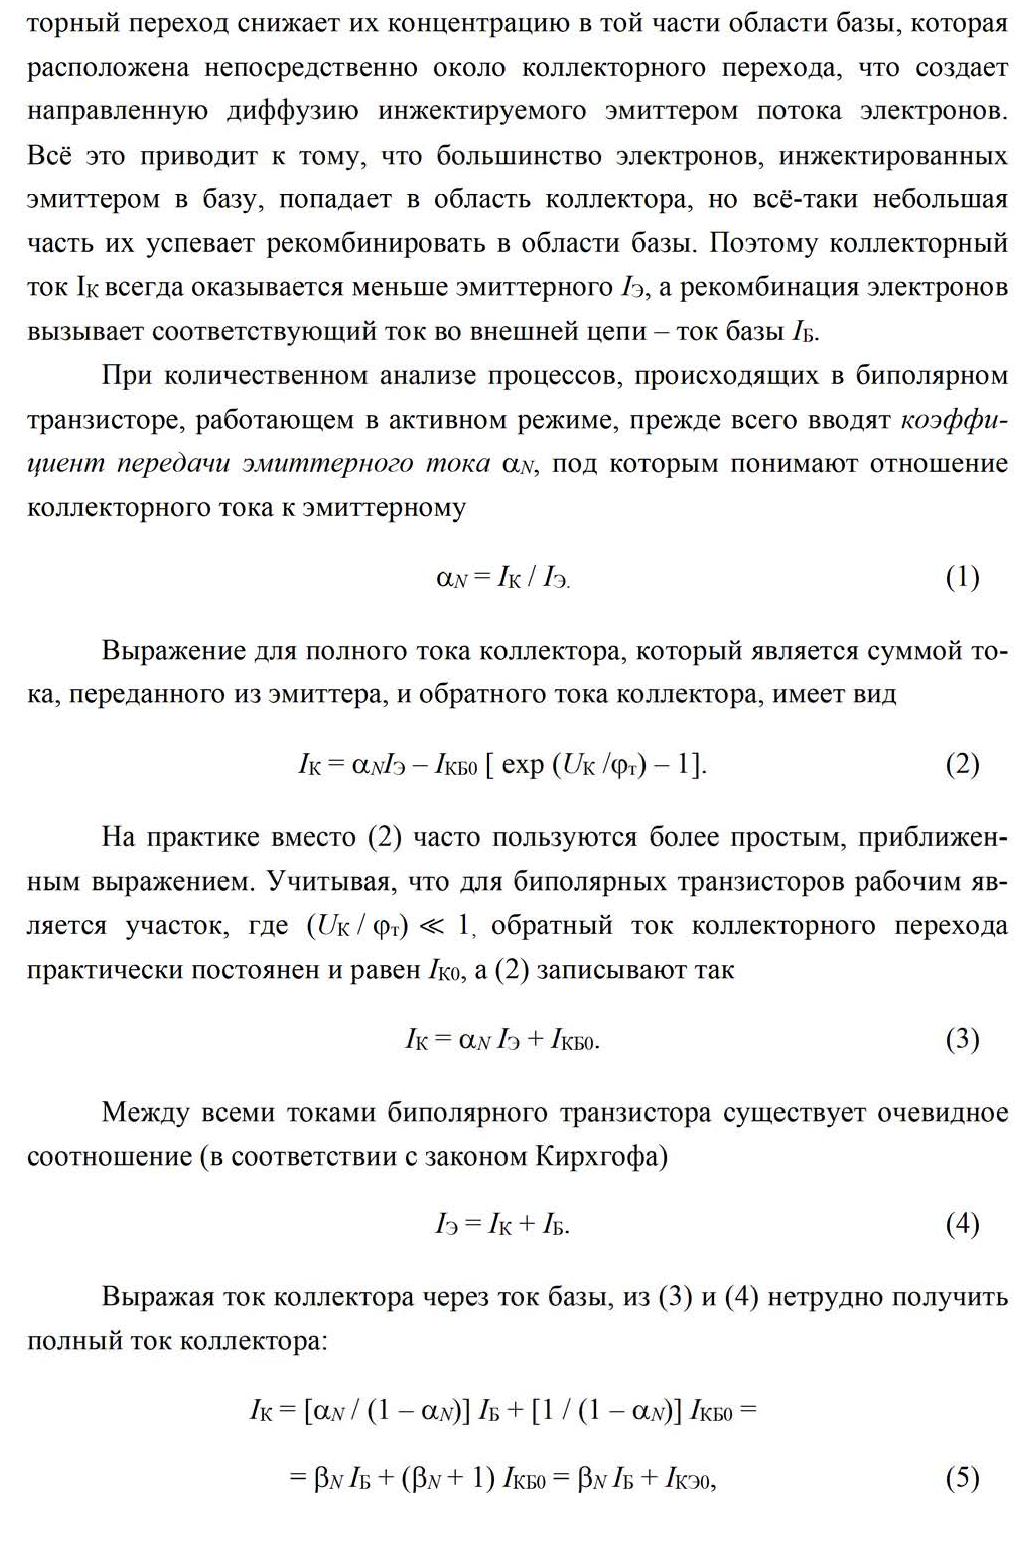
\includegraphics[width=\linewidth]{images/theory_3}
	\caption*{}
	\label{fig:theory3}
\end{figure}

\begin{figure}[H]
	\centering
	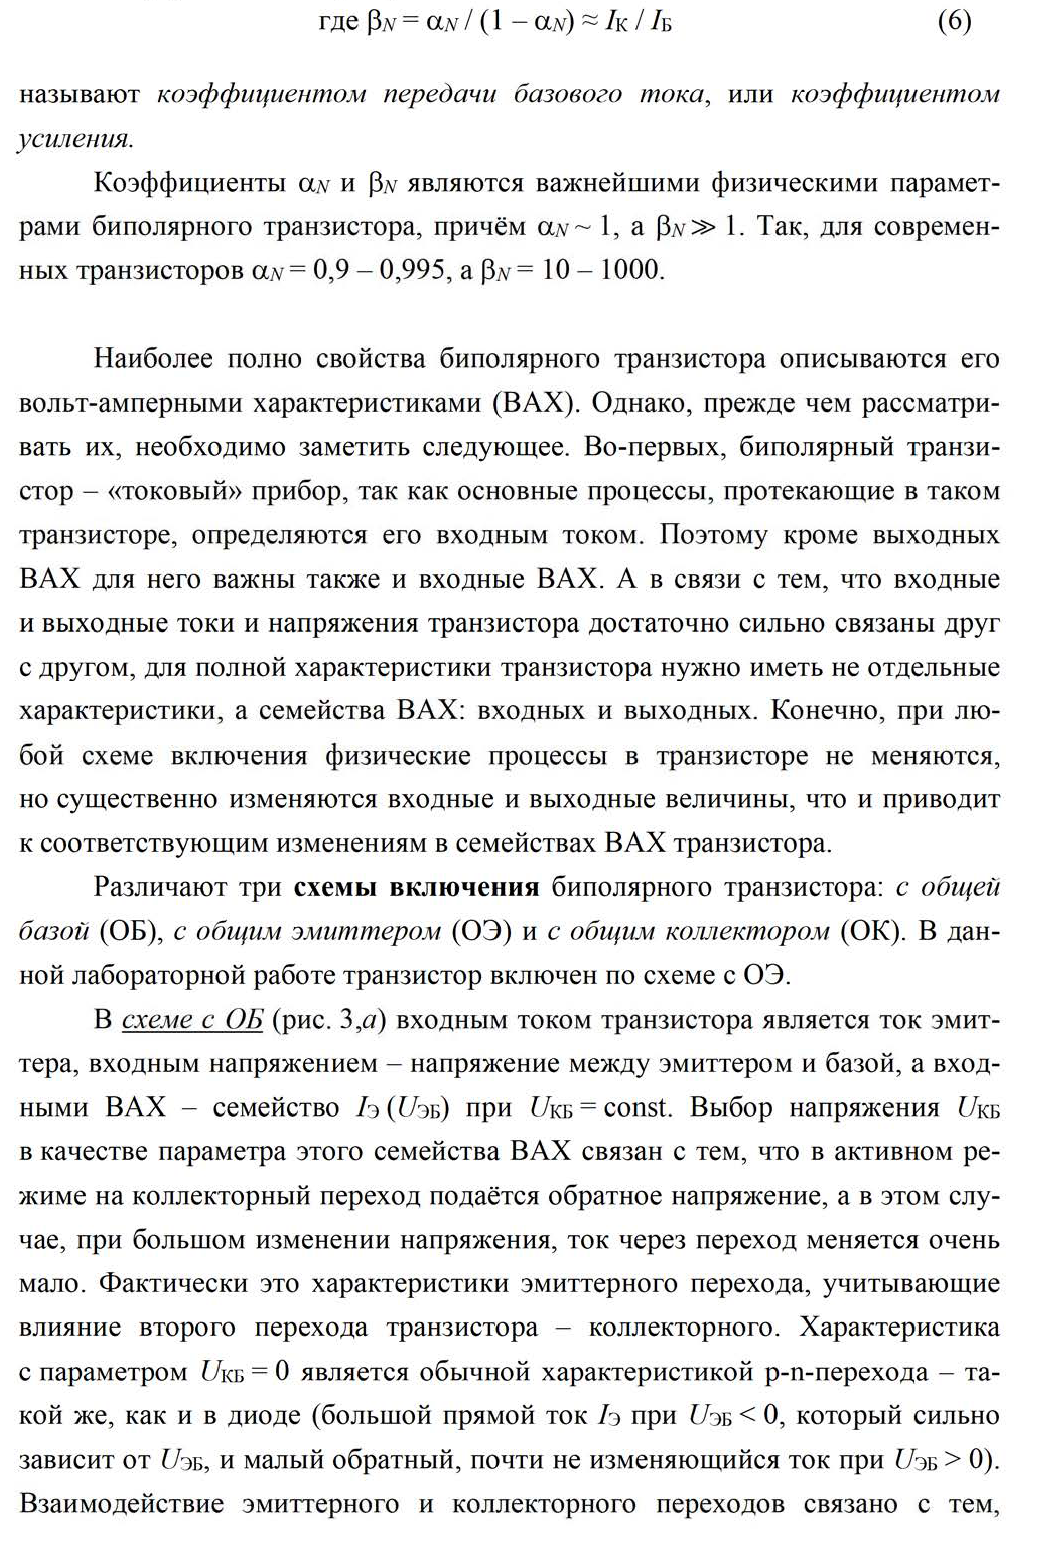
\includegraphics[width=\linewidth]{images/theory_4}
	\caption*{}
	\label{fig:theory4}
\end{figure}

\begin{figure}[H]
	\centering
	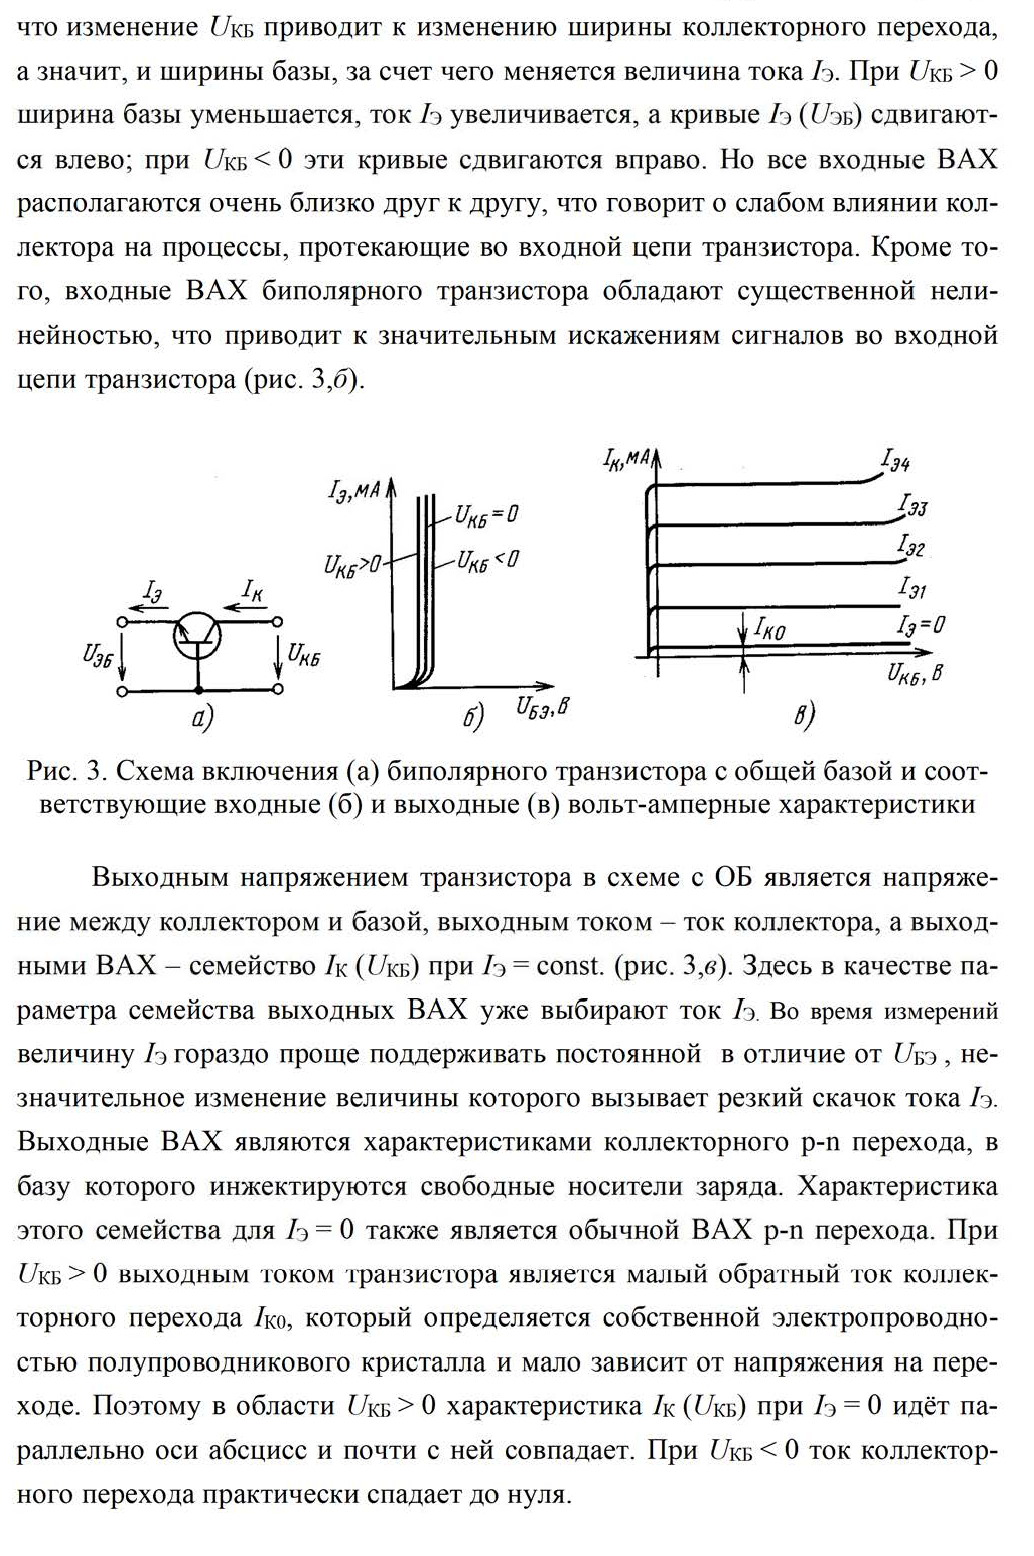
\includegraphics[width=\linewidth]{images/theory_5}
	\caption*{}
\end{figure}

\begin{figure}[H]
	\centering
	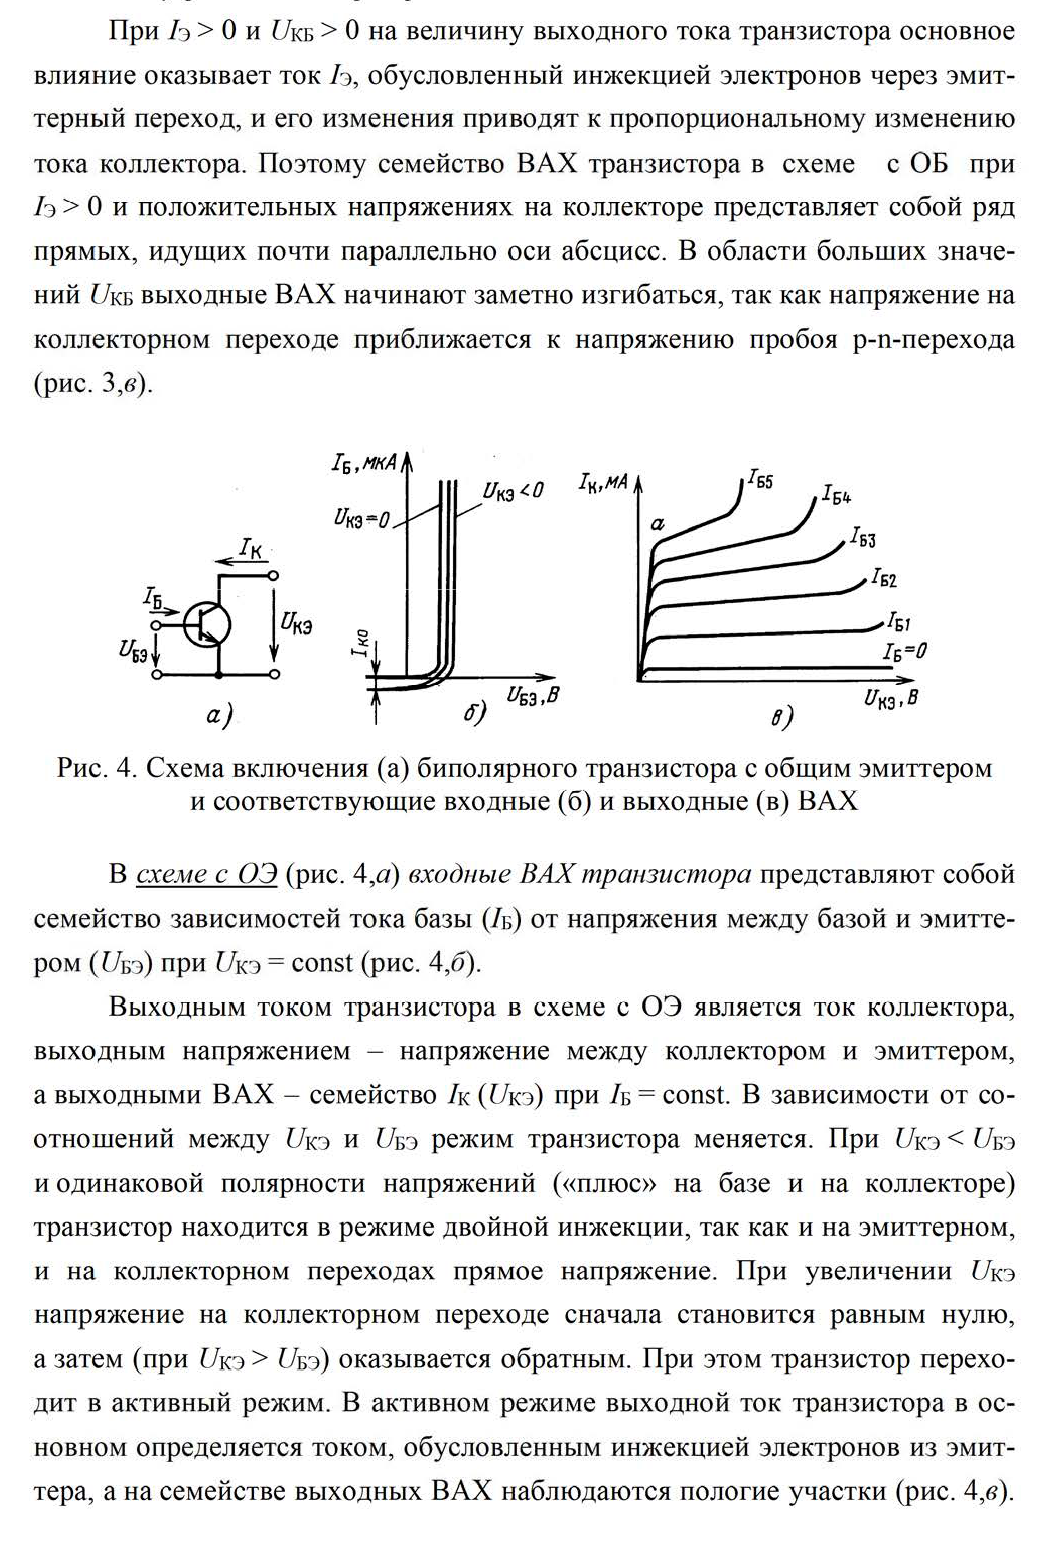
\includegraphics[width=\linewidth]{images/theory_6}
	\caption*{}
\end{figure}

\begin{figure}[H]
	\centering
	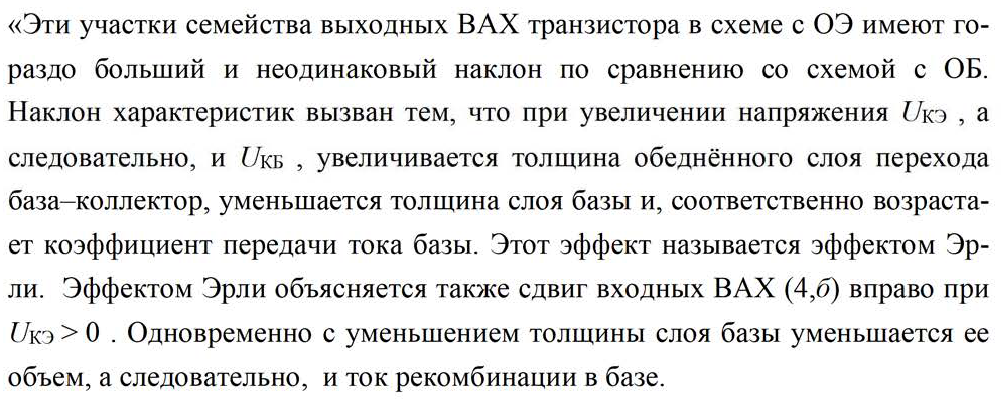
\includegraphics[width=\linewidth]{images/theory_7}
	\caption*{}
\end{figure}

\pagebreak

\section{Схемы измерений}
\begin{figure}[H]
	\centering
	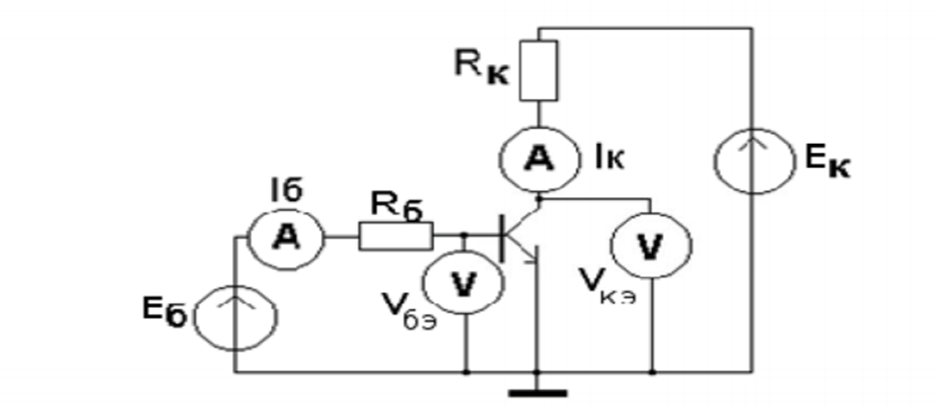
\includegraphics[width=0.7\linewidth]{images/shema}
	\caption{}
	\label{fig:shema}
\end{figure}

\section{Таблицы с результатами измерений}
\subsection{ Задание 1}
\begin{table}[H]
	\begin{tabular}{|c|c|c|}
		\hline
		Uб(В) & Iб(мкА) & Iк(мкА) \\ \hline
		-0.08 & 0.1     & 2.7     \\ \hline
		-0.03 & 0.1     & 4       \\ \hline
		-0.03 & 0.2     & 7.2     \\ \hline
		0.03  & 0.3     & 16.6    \\ \hline
		0.06  & 0.5     & 24.2    \\ \hline
		0.13  & 0.9     & 53.2    \\ \hline
		0.19  & 1.1     & 70.5    \\ \hline
		0.33  & 1.4     & 94      \\ \hline
		0.48  & 2.2     & 150     \\ \hline
		0.52  & 2.6     & 170     \\ \hline
		0.58  & 5       & 400     \\ \hline
		0.64  & 21.4    & 2600    \\ \hline
		0.68  & 156     & 4901    \\ \hline
		0.71  & 655     & 8420    \\ \hline
	\end{tabular}
\end{table}


\subsection{ Задание 2}

\begin{table}[H]
	\begin{tabular}{|c|c|c|c|c|c|}
		\hline
		\multicolumn{2}{|c|}{Iб = 30мкА} & \multicolumn{2}{c|}{Iб = 50мкА} & \multicolumn{2}{c|}{Iб = 70мкА} \\ \hline
		Uк(В)          & Iк(мА)1         & Uк(В)         & Iк(мА)2         & Uк(В)         & Iк(мА)3         \\ \hline
		0.02           & 0               & 0.01          & 0               & 0.01          & 0               \\ \hline
		0.06           & 0.28            & 0.05          & 0.28            & 0.02          & 0.1124          \\ \hline
		0.09           & 0.73            & 0.09          & 1.25            & 0.05          & 0.378           \\ \hline
		0.11           & 1.019           & 0.28          & 6.15            & 0.08          & 1.5             \\ \hline
		0.15           & 1.69            & 0.99          & 6.73            & 0.1           & 2.55            \\ \hline
		0.29           & 3.39            & 1.74          & 6.93            & 0.13          & 4.16            \\ \hline
		0.69           & 3.76            &               &                 & 0.17          & 6.26            \\ \hline
		1              & 3.86            &               &                 & 0.19          & 7.32            \\ \hline
		1.2            & 3.9             &               &                 & 0.5           & 9.2             \\ \hline
		1.5            & 3.95            &               &                 & 0.58          & 9.25            \\ \hline
		1.75           & 4               &               &                 & 0.6           & 9.23            \\ \hline
		1.95           & 4.02            &               &                 &               &                 \\ \hline
		2.23           & 4.08            &               &                 &               &                 \\ \hline
		2.65           & 4.15            &               &                 &               &                 \\ \hline
		3              & 4.19            &               &                 &               &                 \\ \hline
		3.1            & 4.2             &               &                 &               &                 \\ \hline
	\end{tabular}
\end{table}



\section{Графики}

\begin{figure}[H]
	\centering
	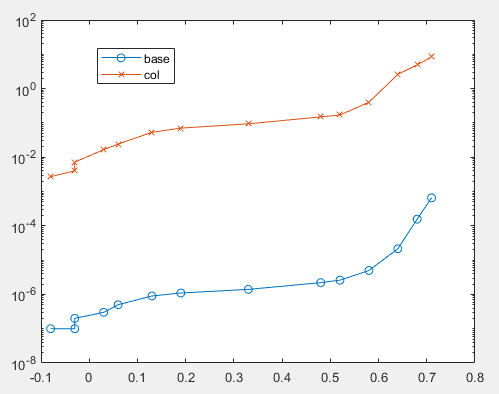
\includegraphics[width=0.7\linewidth]{images/graf11}
	\caption{}
	\label{fig:graf11}
\end{figure}


\begin{figure}[H]
	\centering
	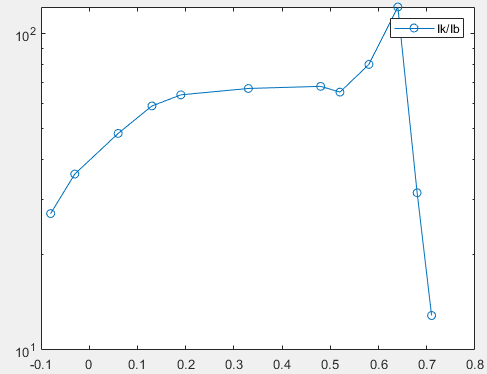
\includegraphics[width=0.7\linewidth]{images/graf3}
	\caption{}
	\label{fig:graf3}
\end{figure}


\begin{figure}[H]
	\centering
	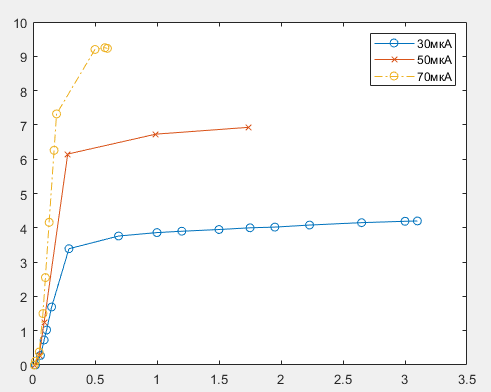
\includegraphics[width=0.7\linewidth]{images/graf1}
	\caption{}
	\label{fig:graf1}
\end{figure}


\section{ Ход и результаты вычисления предварительных значений параметров модели Гуммеля-Пуна по результатам измерений}

$$Rc = \dfrac{0.19}{7.32} * 10^{-3} = 2.596 * 10^{-5} = 259.6Om$$

$$VAF = \dfrac{(3.1 - 0.29)}{4.2 - 3.39} * 3.39 - 0.29 = 12.05B$$ 
 
$$I_{k1} = Is * (exp(\dfrac{U_{be1}}{ nf * fi}) - 1)$$

$$I_{k2} = Is * (exp(\dfrac{U_{be2}}{ nf * fi}) - 1)$$

$$U_{be1} = nf * 0.026 * ln(\dfrac{I_{k1}}{Is})$$

$$U_{be2} = nf * 0.026 * ln(\dfrac{I_{k2}}{Is})$$

$$58 * 10^{-2} = nf * 0.026* ln(\dfrac{400 * 10^{-3}}{Is})$$

$$71 * 10^{-2} = nf * 0.026* ln(\dfrac{8420 * 10^{-3}}{Is})$$

$$Is = 4.99 * 10^{10}$$

$$nf = 1.64$$

$$U_{be3} = nf * 0.026 * ln(\dfrac{I_{k3}}{Is} + 1) + I_{b1} * Rb$$

$$Rb = 108 * 10^4$$

$$Bf = max(\dfrac{I_{k3}}{I_b})$$

Максимум находится при напряжении базы 0,71В

$$Bf = \dfrac{8420}{855} = 12.85$$

\section{Схемы для компьютерного расчета входных и выходных  ВАХ из программы моделирования}

\begin{figure}[H]
	\centering
	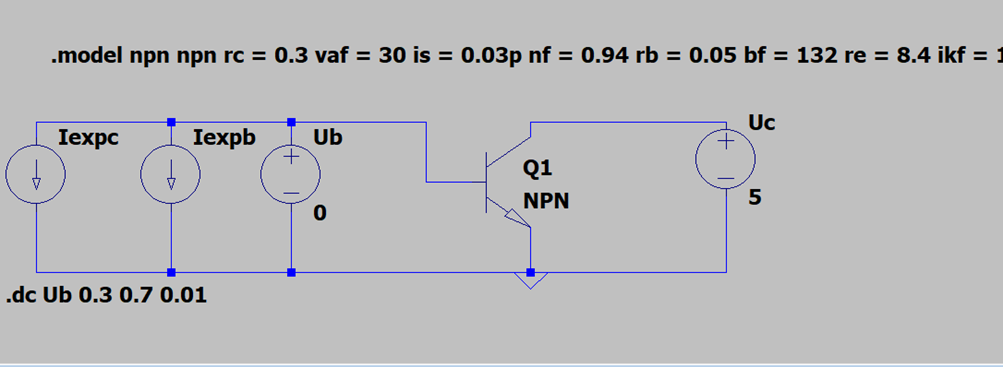
\includegraphics[width=0.7\linewidth]{images/shema1}
	\caption{Схема в LTSpice для расчета входных ВАХ}
	\label{fig:shema1}
\end{figure}

\begin{figure}[H]
	\centering
	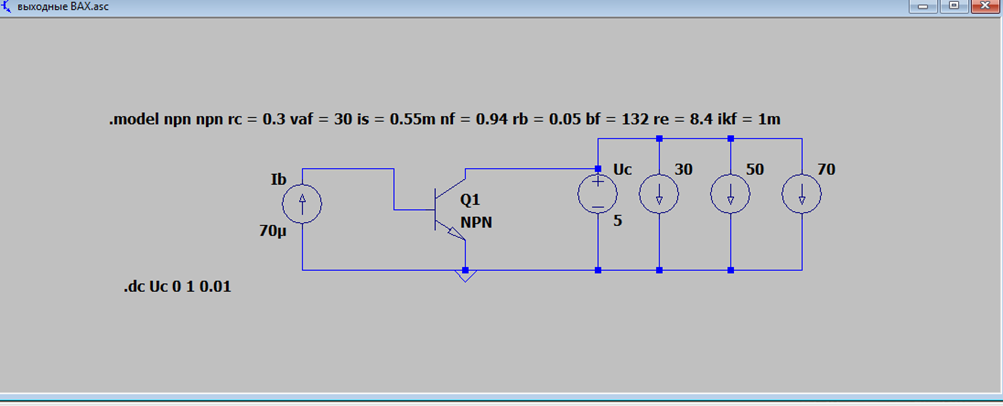
\includegraphics[width=0.7\linewidth]{images/shema2}
	\caption{Схема в LTSpice для расчета выходных ВАХ}
	\label{fig:shema2}
\end{figure}

\section{Графики входных и выходных ВАХ}

\subsection{графики входных ВАХ}
\begin{figure}[H]
	\centering
	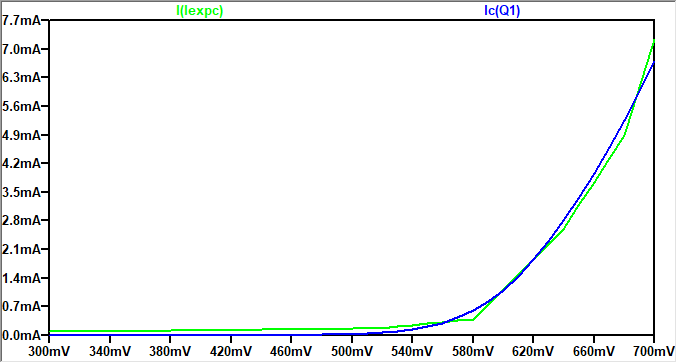
\includegraphics[width=0.7\linewidth]{images/graf8}
	\caption{Зависимость Ic}
	\label{fig:graf8}
\end{figure}


\begin{figure}[H]
	\centering
	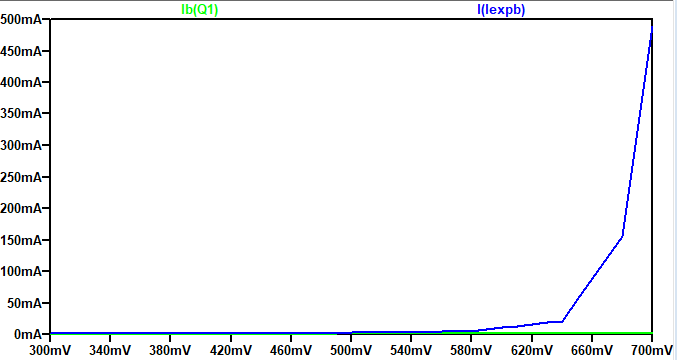
\includegraphics[width=0.7\linewidth]{images/graf9}
	\caption{Зависимость Ib}
	\label{fig:graf9}
\end{figure}

\subsection{графики выходных ВАХ}

\begin{figure}[H]
	\centering
	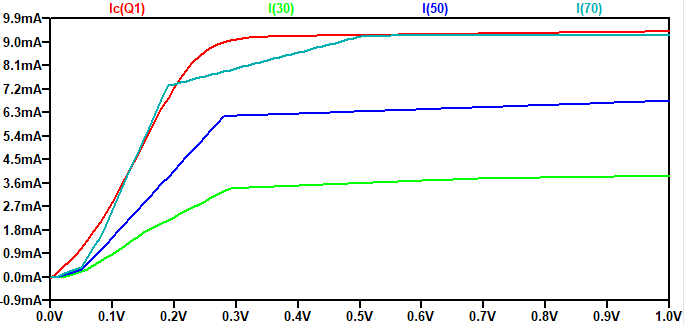
\includegraphics[width=0.7\linewidth]{images/graf10}
	\caption{}
	\label{fig:graf10}
\end{figure}



\end{document} % конец документа

